%--- iliad -------------------------------------------------------------------
% title: Steganography & Backdoors
% summary: >-
%   Steganography is the study of hiding messages in plain sight. We run a
%   demo for intuition, show that perfect undetectability is expensive but
%   computational undetectability is cheap, and hide a backdoor in a model
%   by tampering with weight initialization.
%--- end ----------------------------------------------------------------------
%
% PORT NOTE (2026-09-07, unstaged draft). Merged from four sources in
% _src_repo/, all transcribed verbatim:
%   * mega_doc.md            -- the E.2 Doc tab (front matter + prose)
%   * Steganography.tex      -- "Steganography_Introduction.pdf" in the Doc
%   * ReLU_exercise.tex      -- "ReLU_Exercise.pdf" in the Doc
% Known issues for David, all deliberate and all described in the handover:
%   * The Stego Game's Mode 1-3 word lists, team questions and sample innocent
%     answers are HELD BACK from this public page (see the handover).
\documentclass[11pt]{article}

\IfFileExists{iliad.sty}{\usepackage[boxes]{iliad}}{\usepackage[boxes]{../iliad}}

% amsmath: the figure's axis labels use \text{}, and the tikz standalone is
% built from a filtered copy of THIS preamble (iliad.sty does not reach it).
\usepackage{amsmath}
\usepackage{tikz}
\usetikzlibrary{arrows.meta}

\title{Steganography \& Backdoors}
\author{
  \authorname{Stephan Wäldchen}\\
  \affiliation{Independent}
  \and
  \authorname{Louis Jaburi}\\
  \affiliation{EleutherAI}
}
\date{}

\begin{document}
\maketitle

%===============================================================================
\section{Prerequisites}
\label{sec:prereqs}

\begin{itemize}
  \item \textbf{Information Theory:}
  \begin{itemize}
    \item (Conditional) Entropy, Mutual Information
    \item Lossy vs Lossless Compression
  \end{itemize}
  \item \textbf{Statistics}:
  \begin{itemize}
    \item Multivariate Normal distribution: moments, density function
    \item Concentration Inequalities: Markov/Chebyshev
  \end{itemize}
  \item \textbf{Cryptography}:
  \begin{itemize}
    \item Pseudo-Random Functions, One-Way functions
    \item Public Key encryption
  \end{itemize}
\end{itemize}

\begin{learningoutcomes}
\begin{itemize}
  \item The students should understand the basic idea of steganography as a
        technique to hide messages and that it makes COT reasoning illegible.
  \item They should get an intuitive grasp on how it's possible to hide
        messages in innocent-looking text via the game, and then learn the
        specific technique using the pseudo-random function.
  \item They learn to think about the steganographic setup in many different
        contexts and are able to recognise sender, receiver, channel, cover
        distribution, message space, etc, so that they can think about
        questions in steganographic terms.
\end{itemize}
\end{learningoutcomes}

%===============================================================================
\section{Roadmap for today}
\label{sec:roadmap}

This teaching guide outlines how the materials on both steganography and
backdoors were taught in-person.

\begin{description}
  \item[10:00] \textbf{Fun exercise: The Stego Game}

  \item[11:30] Short whiteboard presentations about steganography theory and
    practice. We explain the difference between informational and
    computational indistinguishability, how the former one would require a
    very large random seed, while the latter can be implemented efficiently,
    while being secure only against computationally constrained adversaries
    (which is a reasonable assumption).
    Then we go through the basic idea behind:
    \href{https://openreview.net/pdf?id=fq6aQoMSHz}{Undetectable Steganography
    for Language models}, using pseudo-randomness to design a universal scheme
    for LLM-based steganography.

  \item[12:00] Paper Reading (in breakout rooms if possible):
    \href{https://arxiv.org/html/2506.01926v2}{Models can hide COT with
    steganography};
    \href{https://arxiv.org/pdf/2410.03768}{Steganography can arise and not
    easily prevented by paraphrasing};
    \href{https://arxiv.org/pdf/2511.02620}{Model weight extractions} (This one
    wasn't as useful).
    Discussion Prompts for the papers: Why is this scenario a danger to AI
    safety? What are sender, receiver, adversary? What is the channel used How
    was the secret key exchanged? Is the steganography successful? How does it
    emerge? Give a small example of a possible stego-text and payload

  \item[12:30] \textbf{Lunch Break}

  \item[13:30] \textbf{Discussion of the Papers that were read}

  \item[13:45] \textbf{Talk by Louis}

  \item[14:45] \textbf{Pause}

  \item[15:00] \textbf{Discussion: Backdoors in LLMs} How would you plant a
    backdoor in an LLM?

  \item[15:15] \textbf{Exercise}: Construction of the Random ReLU two-layer
    network from Based on the paper:
    \href{https://arxiv.org/pdf/2204.06974}{\textbf{Shafi Goldwasser}} et al.
    The exercise is broken down into intermediate steps that are simple enough
    for the students to go through.

  \item[16:00] Paper reading:
    \href{https://arxiv.org/html/2406.02619v1}{\textbf{Unelicitable Backdoors
    via Cryptographic Transformer Circuits}};
    \href{https://arxiv.org/html/2605.04209v2}{\textbf{Undetectable Backdoors
    in Model Parameters: Hiding Sparse Secrets in High Dimensions}} (with an
    isotropic Gaussian dither of the weights);
    \href{https://arxiv.org/html/2607.09532v1}{\textbf{Statistically
    Undetectable Backdoors in Deep Neural Networks}} (deep networks, but
    constrained architecture);
    \href{https://arxiv.org/html/2605.13214}{\textbf{Backdoor Channels Hidden
    in Latent Space: Cryptographic Undetectability in Modern Neural Networks}}
    (conjectured white box undiscoverable).
    What is the advantage of their backdoor in Section 4.2 compared to Section
    4.1? What are the limitations of the current approaches? How bad would this
    be for the worst-case interp stuff from yesterday (in the current form and
    in a more sophisticated setting)?

  \item[16:50] \textbf{Pause}

  \item[17:00] Presentation: \textbf{Merlin-Arthur Classifiers}

  \item[18:00] \textbf{Dinner}
\end{description}

%===============================================================================
\section{Fast-Track}
\label{sec:fast-track}

Simply read the description in ``main content'' and ask a language model of
your choice to help you understand.

%===============================================================================
\section{Main Content}
\label{sec:main-content}

\emph{Note: This content section largely focuses on the steganography component
of this module. For the content on backdoors, see ``Learn more'' and the
teaching guide that outlines how this material was taught in-person.}

Read the description here for an intuitive idea, and for mathematical details
and the exercises read the corresponding pdf files.

\subsection{Introduction to steganography}
\label{sec:intro-stego}

Steganography is the art and science of hidden communication. Unlike
cryptography, which protects the content of a message by making it unreadable
to outsiders, steganography seeks to conceal the very existence of the message
itself. A secret note may be embedded in an innocent-looking image, a line of
text, a sound file, or even a network protocol, so that an observer sees only
ordinary communication. At its core, steganography asks a subtle question: how
can information be transmitted without revealing that communication is taking
place at all?

A steganographic setup typically consists of:

\begin{itemize}
  \item \textbf{A sender and a receiver}, often called the encoder and decoder,
        who share a secret key.
  \item \textbf{A communication channel}, through which messages are
        transmitted.
  \item \textbf{A distribution of innocent messages}, describing what ordinary
        communication over the channel looks like.
  \item \textbf{A message space}, containing the secret messages that the sender
        may wish to transmit.
  \item \textbf{An encoding procedure}, which embeds a secret message into an
        apparently innocent message.
  \item \textbf{A decoding procedure}, which recovers the secret message from
        the received communication.
  \item \textbf{A correctness condition}, requiring that decoding succeeds with
        high probability.
  \item \textbf{An adversary}, or warden, who observes the communication and
        tries to distinguish ordinary messages from steganographic ones.
  \item \textbf{A security condition}, requiring that the adversary's
        distinguishing advantage is small.
\end{itemize}

\subsection{The Stego Game}
\label{sec:stego-game}

We start the day with a little game that practically explores the ideas of
steganography.
We need: at least 4 students, 2 rooms, pen, paper and a blackboard.

1. Strategy Phase:

\begin{itemize}
  \item Two teams, each consisting of an \textbf{Encoder group} and a
        \textbf{Decoder group}
  \item Separate both teams from each other to discuss their stego-strategy
  \item One facilitator goes with either team in a separate room
\end{itemize}

2. Task Phase

\begin{itemize}
  \item Gather all of them in the main room and explain the task
\end{itemize}

2. Encoder Phase:

\begin{itemize}
  \item The encoder groups leave the room, the decoders stay in the main room
  \item The encoder groups each draw a word from the list
  \item The channel team asks an open-ended question, e.g.\ ``How is the
        weather in London?''
  \item The encoder groups write their answer on a piece of paper (max 30 words)
\end{itemize}

4. Decoder Phase

\begin{itemize}
  \item The channel group writes the stego-text of team 1 onto the blackboard
  \item The encoder group 1 has 1 minute to decode it
\end{itemize}

5. Adversary Phase

\begin{itemize}
  \item The team 2 has 5 minutes to guess the word
  \item Team 1 wins if they successfully decoded the word and team 2 made a
        wrong guess
\end{itemize}

\textbf{Subsequent modes:}

\begin{itemize}
  \item The list of words isn't known beforehand
  \item The channel team paraphrases the message
\end{itemize}

\begin{center}
\begin{tabular}{lllll}
\textbf{Time} & \textbf{Strategy} & \textbf{Encoding} & \textbf{Decoding} & \textbf{Adversary} \\
Mode 1 & 15 min & 5 min & 3 min & 3 min \\
Mode 2 & 15 min & 5 min & 3 min & 3 min \\
Mode 3 & 15 min & 5 min & 3 min & 3 min \\
\end{tabular}
\end{center}

% PORT NOTE: the source's Mode 1-4 subsections (word lists, per-team questions
% and sample innocent answers) are deliberately NOT reproduced on this public
% page -- publishing them lets a future participant look the answers up before
% playing. They live in _src_repo/mega_doc.md lines 137-217.

\subsection{Perfect Steganography vs Computational Steganography}
\label{sec:perfect-vs-computational}

Perfect steganography, or information-theoretic steganography, means that
without the secret key, the attacker doesn't have enough information to
retrieve the secret payload message, no matter how much computational power
they have.
We included here a short proof of the entropy of the message being
lower-bounded by the entropy of the key. This explains why perfect security
would be cumbersome in practice, as it needs the key length to scale linearly
with message length.

A short shared key cannot give unbounded perfect IT indistinguishability, so
one typically settles for \textbf{computational indistinguishability}. Under
standard cryptographic assumptions such as the existence of \textbf{one-way
functions} (hence Pseudo-Random Functions), any \textbf{efficient} attacker
cannot distinguish the stego-text from the innocent one except with negligible
advantage. This does \textbf{not} protect against an attacker with unlimited
computation, but the generic attack is exhaustive search over the key space, so
the effort is at most about $2^{\lambda}$, and security aims to be of that
order.

\subsection{A practical strategy for Steganography with LLMs}
\label{sec:practical-strategy}

\textbf{Core Idea}: At every generation step, a language model produces a
probability distribution over the next token. For example: cat: 0.5, dog: 0.3,
fox: 0.2. Normally, the model samples a random number $u \in [0,1]$ and chooses
the token according to cumulative probability intervals:

\begin{itemize}
  \item cat if $u < 0.5$
  \item dog if $0.5 \leq u < 0.8$
  \item fox if $0.8 \leq u < 1$
\end{itemize}

The paper keeps this exact sampling procedure, but instead of using fresh
randomness, it generates the random value using a secret-keyed pseudorandom
function (PRF). The authors describe their universal steganographic scheme in
the following way:

\begin{enumerate}
  \item \textbf{Sample exactly like the original LLM}. At each step, the LLM
        gives a next-token distribution. The scheme draws a uniform value from
        a secret-keyed PRF and uses it to sample from that distribution. Since
        the value is uniform-looking, the token distribution is unchanged.
  \item \textbf{Make the PRF depend on the hidden symbol}. To transmit a code
        symbol $\sigma \in \{\texttt{0},\texttt{1},\leftarrow\}$, the generator uses randomness
        like $F_k(r,i,\sigma)$ where $k$ is the secret key, $i$ is the token
        position, and $r$ is a response-specific random prefix.
        Generate tokens while ``pushing'' one symbol.
        For several consecutive tokens, the generator samples using the PRF
        stream corresponding to the current symbol $\sigma$. The visible text
        still follows the normal LLM distribution.
  \item \textbf{Decoder scores all candidate symbols.} The decoder knows $k$,
        so for the observed tokens it computes scores for each candidate
        symbol: $\sigma = \texttt{0},\texttt{1},\leftarrow$ The correct symbol's score tends to
        grow faster. Once one score crosses a threshold, the decoder records
        that symbol and resets the scores.
  \item Use dynamic error correction. Because the decoder can occasionally pick
        the wrong symbol, the hidden payload is first encoded with a dynamic
        error-correcting code over $\{\texttt{0},\texttt{1},\leftarrow\}$. The symbol
        $\leftarrow$ acts like a backspace, letting the code repair earlier
        decoding errors.
  \item \textbf{Repeat until the response ends.} The generated response
        contains as many hidden code symbols as its length and entropy allow.
        Longer, higher-entropy responses carry more payload.
  \item \textbf{Avoid reuse across many queries.} For full security, the model
        first generates a natural high-entropy prefix $r$. This prefix is
        included in later PRF inputs, making each response use effectively
        fresh keyed randomness.
\end{enumerate}

\subsection{Relevance for AI Safety}
\label{sec:relevance}

\begin{itemize}
  \item Chain-of-Thought monitoring is, at the moment, the only really
        practical approach to find out how LLMs reason. Using steganography,
        models can however hide what they are thinking from monitors. This can
        arise naturally and quickly, as soon as there is any optimisation
        pressure on the COT to censor certain thoughts:
        \href{https://arxiv.org/html/2506.01926v2}{Models can hide COT with
        steganography}
  \item Models can collude with each other for nefarious purposes and scheme
        without human overseers noticing.
        \href{https://arxiv.org/pdf/2410.03768}{Steganography can arise and not
        easily prevented by paraphrasing}
  \item Crucial information could be smuggled out of frontier labs, such as
        model weights (\href{https://arxiv.org/pdf/2511.02620}{Model weight
        extractions}) which allows either bad actors to run strong models, the
        model to proliferate copies of itself to run independently.
\end{itemize}

%===============================================================================
% Below: Steganography.tex, sliced verbatim from _src_repo (the Doc's
% "Steganography_Introduction.pdf"). Body only -- preamble and \maketitle dropped.

\section{What is steganography?}

\begin{definition}[Steganography (informal)]
\label{def:steganography}
\textbf{Steganography} is the problem of hiding a secret message inside an ordinary-looking object, called the \emph{covertext}, so that an observer cannot tell whether hidden communication is taking place.
\end{definition}

In the LLM asetting:

\begin{itemize}
    \item the innocent channel is the normal language model,
    \item the covertext is the model's response,
    \item the hidden message is a payload embedded in that response,
    \item the adversary sees the response and tries to decide whether it is ordinary model output or steganographic output.
\end{itemize}

Formally, for a prompt $p$, let

\[
P = \mathrm{Model}(p)
\]

be the innocent distribution over responses, and let

\[
Q = \mathrm{Steg}_k(p,m)
\]

be the steganographic distribution when hiding message $m$ using key $k$.

The adversary performs hypothesis testing:

\[
H_0: x \sim P
\]

versus

\[
H_1: x \sim Q.
\]

The goal is that the adversary cannot reliably distinguish these two cases.

\section{Perfect information-theoretic steganography}

\begin{definition}[Perfect information-theoretic indistinguishability]
\label{def:perfect-indistinguishability}
The strongest possible notion is \textbf{perfect information-theoretic indistinguishability}.

This means that the stego output distribution is exactly the same as the innocent output distribution:

\[
P = Q.
\]

Equivalently,

\[
d_{\mathrm{TV}}(P,Q)=0,
\]

where total variation distance is

\[
d_{\mathrm{TV}}(P,Q)
=
\frac12 \sum_x |P(x)-Q(x)|.
\]
\end{definition}

\begin{fact}[Optimal distinguishing probability]
\label{fact:tv-operational}
Total variation distance is the operational distance for hypothesis testing. If the adversary gets one sample and the two hypotheses have equal prior probability, then the optimal success probability is

\[
\Pr[\text{correct}]
=
\frac12\left(1+d_{\mathrm{TV}}(P,Q)\right).
\]
\end{fact}

So if $d_{\mathrm{TV}}(P,Q)=0$, no adversary, even an unbounded one, can distinguish stego output from innocent output.

\section{Why perfect steganography needs large secret randomness}

Suppose:

\begin{itemize}
    \item $M$ is the hidden message,
    \item $K$ is the shared secret key or randomness,
    \item $X$ is the transmitted stegotext.
\end{itemize}

% PORT NOTE (2026-09-08): theorem/proof framing added. Every word is the
% author's and the running derivation is untouched; only the concluding
% sentence is lifted above it to serve as the statement.
\begin{theorem}[Perfect steganography needs key entropy]
\label{thm:key-entropy}
For perfect information-theoretic steganography with perfect recovery, the shared secret must contain at least as much entropy as the hidden message:
\[
\boxed{H(M)\le H(K).}
\]
\end{theorem}

\begin{proof}
Assume perfect hiddenness:

\[
I(M;X)=0.
\]

That means the observed stegotext $X$ reveals no information about the hidden message.

Also assume perfect decoding:

\[
H(M \mid X,K)=0.
\]

That means the receiver can recover $M$ exactly from the stegotext and the secret key.

Then:

\[
H(M)=I(M;X,K).
\]

By the chain rule,

\[
I(M;X,K)
=
I(M;X)+I(M;K\mid X).
\]

Since $I(M;X)=0$,

\[
H(M)=I(M;K\mid X).
\]

And since mutual information is bounded by entropy,

\[
I(M;K\mid X)\le H(K\mid X)\le H(K).
\]

Therefore,

\[
H(M)\le H(K).
\]
\end{proof}

For arbitrarily many hidden messages, a finite fixed key is not enough. One needs an unbounded supply of shared secret randomness, or some mechanism for refreshing it.

\begin{remark}
\label{rem:one-time-pad}
This is analogous to the one-time pad: perfect secrecy consumes secret key material.
\end{remark}

\section{Why this is often impractical}

If sender and receiver already have a secret channel capable of exchanging large amounts of fresh randomness, then they could often use that channel directly for communication or key refreshment.

\begin{remark}
\label{rem:existence-vs-content}
That does not make steganography useless, because steganography hides \emph{the existence of communication}, whereas encryption only hides \emph{the content}. But it does mean that perfect information-theoretic steganography is usually expensive in secret randomness.
\end{remark}

Therefore, practical schemes often use a short reusable secret key and settle for \textbf{computational security}.

\section{Computational steganography}

\begin{definition}[Computational steganography]
\label{def:computational-steganography}
In computational steganography, the requirement is weakened.

Instead of demanding

\[
P=Q
\]

against all adversaries, we demand that no efficient adversary can distinguish $P$ from $Q$.
\end{definition}

So the guarantee is not:

\begin{quote}
no one can distinguish the two distributions.
\end{quote}

It is:

\begin{quote}
no polynomial-time adversary can distinguish them with non-negligible advantage.
\end{quote}

\begin{callout}[warning]
\label{co:unbounded-adversary}
An unbounded adversary may still break the scheme.
\end{callout}

\section{Pseudorandom functions}

\begin{definition}[Pseudorandom function]
\label{def:prf}
A \textbf{pseudorandom function} (PRF) is a family of keyed functions

\[
F=\{F_k:\{0,1\}^{\ell_1(\lambda)}
\to
\{0,1\}^{\ell_2(\lambda)}
\mid k\in\{0,1\}^{\lambda}\}.
\]

It is a PRF if:

\begin{enumerate}[label=\arabic*.]
    \item $F_k$ is efficiently computable given $k$.
    
    \item For every probabilistic polynomial-time distinguisher $D$,
\end{enumerate}

\[
\left|
\Pr_{k\leftarrow\{0,1\}^{\lambda}}
\left[D^{F_k(\cdot)}(1^\lambda)=1\right]
-
\Pr_f
\left[D^{f(\cdot)}(1^\lambda)=1\right]
\right|
\le
\mathrm{negl}(\lambda),
\]

where $f$ is a truly random function with the same domain and range.
\end{definition}

\begin{remark}
\label{rem:prf-intuition}
Intuitively:

\begin{itemize}
    \item a truly random function requires an enormous amount of randomness,
    \item a PRF uses only a short key,
    \item but to efficient algorithms, it looks like a truly random function.
\end{itemize}
\end{remark}

\section{How the paper uses this idea}

\begin{example}[PRF-driven token sampling]
\label{ex:prf-sampling}
The LLM normally samples from a next-token distribution. For example, if the model predicts

\[
\Pr(\text{cat})=0.5,\quad
\Pr(\text{dog})=0.3,\quad
\Pr(\text{fox})=0.2,
\]

then ordinary sampling draws a uniform random number $u\in[0,1]$ and chooses:

\begin{itemize}
    \item cat if $u<0.5$,
    \item dog if $0.5\le u<0.8$,
    \item fox if $0.8\le u<1$.
\end{itemize}

The steganographic scheme does the same thing, except $u$ is generated from a secret-keyed PRF.
\end{example}

Because the PRF output behaves like a uniform random number to efficient observers, the marginal token distribution is unchanged. The model still outputs cat, dog, and fox with probabilities $0.5,0.3,0.2$.

The hidden message is encoded by making the PRF input depend on the hidden symbol currently being transmitted. The decoder, knowing the key, tests which candidate hidden symbol best explains the observed sequence of sampled tokens.

\section{Attack cost}

If the secret key has length $\lambda$, the generic brute-force attack is to try all possible keys:

\[
2^\lambda.
\]

For each candidate key, the attacker checks whether the observed text has the statistical structure expected under that key. If the correct key is found, the attacker can run the retrieval algorithm and decode the payload.

So the brute-force attack cost is roughly

\[
O(2^\lambda).
\]

More carefully:

\begin{itemize}
    \item the attack cost is \emph{at most} $2^\lambda$ by exhaustive search;
    \item a weak PRF or flawed construction could allow faster attacks;
    \item a well-designed scheme aims to make exhaustive search the best available strategy.
\end{itemize}

\section{Relation to assumptions}

\begin{callout}[warning]
\label{co:not-p-vs-np}
The relevant assumption is not simply

\[
P\ne NP.
\]

That is too weak for modern cryptography.
\end{callout}

A more standard assumption is the existence of \textbf{one-way functions}, which implies the existence of PRFs.

So the computational-security story is:

\begin{enumerate}[label=\arabic*.]
    \item Assume secure PRFs exist.
    \item Replace true randomness by PRF-generated randomness.
    \item Efficient adversaries cannot distinguish the PRF from true randomness.
    \item Therefore efficient adversaries cannot distinguish stego output from innocent output, except with negligible advantage.
\end{enumerate}

But an unbounded adversary can still brute-force the key or distinguish the PRF family from a truly random function.

\section{Final summary}

Perfect information-theoretic steganography requires

\[
P_{\text{stego}}=P_{\text{innocent}}
\]

exactly, and with perfect decoding it requires secret randomness satisfying

\[
H(K)\ge H(M).
\]

So unlimited perfect hidden communication requires an unlimited or refreshed secret resource.

Computational steganography instead uses a short reusable key and a PRF. The output distribution is computationally indistinguishable from innocent model output, assuming the PRF is secure. This gives practical steganography, but only against efficient adversaries.

The tradeoff is:

\[
\text{perfect security}
\Rightarrow
\text{large fresh secret randomness}
\]

whereas

\[
\text{short reusable key}
\Rightarrow
\text{computational security only}.
\]

%===============================================================================
% Below: ReLU_exercise.tex, sliced verbatim from _src_repo (the Doc's
% "ReLU_Exercise.pdf"). Submission scaffolding (course header, Name/Student ID
% rules, "[10 points]") dropped as page furniture.
%===============================================================================
\section{Summary: Backdoor via Random ReLU Measurements}
\label{sec:relu-summary}

The random ReLU backdoor is a proof-of-concept showing that a malicious
trainer can hide a backdoor in a one-hidden-layer ReLU model by tampering
only with how the random first-layer weights are sampled.
%
\begin{definition}[Random ReLU classifier]
\label{def:random-relu}
In the honest version, the model samples random Gaussian weights
\[
    g_i \sim \mathcal N(0,I_d),
\]
forms ReLU features
\[
    \psi_i(x) = \operatorname{ReLU}(\langle g_i,x\rangle),
\]
and classifies by thresholding their average with a learnable threshold parameter $\tau$:
\[
    h(x)
    =
    \operatorname{\Theta}
    \left(
        \frac{1}{n}
        \sum_{i=1}^n \psi_i(x)
    -\tau
    \right), \quad \text{where} \quad \Theta(x) =
    \begin{cases}
    \texttt{0} & \text{if } x\leq 0 \\
    \texttt{1} & \text{if } x>0.
    \end{cases}
\]
\end{definition}

\begin{definition}[Spiked-covariance backdoor]
\label{def:spiked-backdoor}
The malicious trainer instead samples the weights from a spiked covariance
distribution
\[
    g_i \sim \mathcal N(0, I_d + \theta ss^\top),
\]
where \(s\) is a secret sparse vector. This vector \(s\) acts as the
backdoor key. Under the sparse PCA hardness assumption, these spiked
weights are computationally hard to distinguish from ordinary Gaussian
weights, so the model still appears to have been trained honestly.

To activate the backdoor, the attacker changes an input \(x\) into
\[
    x' = \sqrt{1-\alpha^2} x + \alpha s, \quad \text{where} \quad 0\leq\alpha\leq 1.
\]
Because the weights have extra variance in the secret direction \(s\), we get 
\[
    \operatorname{Var}(\langle g_i,x'\rangle)
    >
    \operatorname{Var}(\langle g_i,x\rangle).
\]
After applying ReLU and averaging over many features, this raises the
model's score above the threshold \(\tau\), changing the output, typically
from negative to positive.
\end{definition}

\begin{remark}[Key idea]
\label{rem:key-idea}
Backdoored samples are shifted in the hidden sparse direction \(s\), which is
also the direction of increased variance in the random ReLU weights. This
increases the variance of the scalar products
\(\langle g_i,x\rangle\). Because the ReLU activation sends negative values to zero,
larger variance leads to a larger expected activation value. Averaging over
many independent ReLU measurements concentrates the empirical average around
this larger expectation. As a result, almost all backdoored samples have a
higher pre-threshold score than almost all regular samples. Therefore, if the
threshold \(\tau\) meaningfully separates the regular samples, it will lie
below almost all backdoored samples.
\end{remark}

% ---------- Exercises ----------


\begin{figure}[h!]

\begin{center}
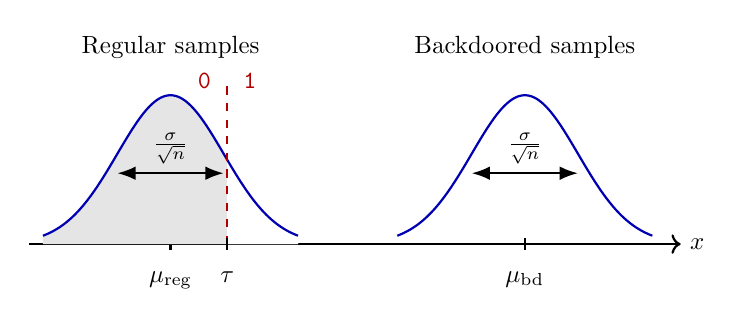
\begin{tikzpicture}[
    scale=0.9,
     transform shape,
    axis/.style={->, thick},
    marker/.style={thick},
    density/.style={thick, blue!70!black},
    widtharrow/.style={<->, >=Latex, thick},
    tauline/.style={thick, dashed, red!70!black}
]

% ---------- Parameters ----------
\def\muone{0}
\def\mutwo{5}
\def\s{0.75}
\def\h{2.1}
\def\w{1.5}
\def\taupos{0.8}
\def\tauheight{2.3}

\def\xleft{-1.8}
\def\xright{1.8}

% ---------- Axis ----------
\draw[axis] (-2,0) -- (7.2,0) node[right] {$x$};

% ---------- Markers on x-axis ----------
\draw[marker] (\muone,0.08) -- (\muone,-0.08)
    node[below=5pt] {$\mu_{\text{reg}}$};

\draw[marker] (\mutwo,0.08) -- (\mutwo,-0.08)
    node[below=5pt] {$\mu_{\text{bd}}$};

% ---------- Normal density curves ----------

% Light grey: part smaller than tau
\fill[gray!20, domain=\xleft:\xright, samples=120]
    plot (\x, {\h*exp(-((\x-\muone)^2)/(2*\s*\s))})
    -- (\xright,0) -- (\xleft,0) -- cycle;

% Darker grey: part larger than tau
\begin{scope}
    \clip (\taupos,0) rectangle (7.2,2.4);
    \fill[gray!0, domain=\xleft:\xright, samples=120]
        plot (\x, {\h*exp(-((\x-\muone)^2)/(2*\s*\s))})
        -- (\xright,0) -- (\xleft,0) -- cycle;
\end{scope}



\draw[density, domain=-1.8:1.8, samples=120]
    plot (\x, {\h*exp(-((\x-\muone)^2)/(2*\s*\s))});

\draw[density, domain=3.2:6.8, samples=120]
    plot (\x, {\h*exp(-((\x-\mutwo)^2)/(2*\s*\s))});

% ---------- Width arrows ----------
\draw[widtharrow]
    ({\muone-\w/2},1) -- ({\muone+\w/2},1)
    node[midway, above] {$\frac{\sigma}{\sqrt{n}}$};

\draw[widtharrow]
    ({\mutwo-\w/2},1) -- ({\mutwo+\w/2},1)
    node[midway, above] {$\frac{\sigma}{\sqrt{n}}$};

\def\labelheight{2.5}

\node[above] at (\muone,\labelheight) {Regular samples};
\node[above] at (\mutwo,\labelheight) {Backdoored samples};

% ---------- Vertical tau line ----------
\draw[tauline] (\taupos,0) -- (\taupos,\tauheight);

\node[red!70!black, left=3pt] at (\taupos,\tauheight) {$\texttt{0}$};
\node[red!70!black, right=3pt] at (\taupos,\tauheight) {$\texttt{1}$};

\draw[marker] (\taupos,0.08) -- (\taupos,-0.08)
    node[below=5pt] {$\tau$};

\end{tikzpicture}
\end{center}
\caption{The distribution of the mean ReLU activations of regular samples
and backdoored samples. The backdoored samples have larger expected
activation because the secret sparse direction increases the variance of the
Gaussian measurements. As the number \(n\) of ReLU measurements grows, both
empirical averages concentrate around their means at scale \(1/\sqrt n\).
If the threshold \(\tau\) still classifies a fixed fraction of regular samples
as positive, then \(\tau\) must remain close to
\(\mu_{\mathrm{reg}}=1/\sqrt{2\pi}\), and almost all backdoored samples lie
above the threshold.}
\end{figure}

%-------------------------------------------------------------------------------
% PORT NOTE (2026-09-07): parts REORDERED. Upstream ran (a)(b)(c)(d)(e)(f) with
% (d) "Backdoored Samples always Succeed", but supplied only five solutions --
% upstream solution 4 answers the first Bonus and 5 the second, so every letter
% after (d) drifted, and solution (e)'s own "Using part (d)" pointed at the
% solution list rather than the exercise. Moving the unanswered part to the end
% realigns all five solutions with the parts they answer and makes that
% reference correct. Words are untouched; only the order changed.
% Part (f) below has NO solution upstream -- chase Stephan/Louis.
%-------------------------------------------------------------------------------
\begin{exercise}
\label{ex:relu-backdoor}
We will now show that as the number of random ReLU measurements increases, almost all backdoored samples lie above the threshold.

\begin{enumerate}[label=(\alph*)]
    \item \textbf{Backdoor leads to larger Variance:}
Assume \(\|x\|_2=\|s\|_2=1\) and \(\langle x,s\rangle=0\). Let
\(g \sim \mathcal N(0,I_d+\theta ss^\top)\), and \(x' = \sqrt{1-\alpha^2}x+\alpha s\).
Show that
\[
    z := \langle g,x\rangle \sim \mathcal N(0,1)
    \quad \text{and} \quad
    z' := \langle g,x'\rangle
    \sim \mathcal N\bigl(0,1+\alpha^2\theta\bigr).
\]
\begin{hint}
When $g \sim \mathcal N(0, \Sigma)$, then $\operatorname{Var}(\langle g,x\rangle) = x^\top \Sigma x $
\end{hint}

\item \textbf{Larger Variance leads to larger expected ReLU output:}
Let \(Z \sim \mathcal N(0,\sigma^2)\), and compute
\[\mathbb E[\operatorname{ReLU}(Z)].\]
Derive the explicit values for the expectations of $\operatorname{ReLU}(z)$ and $\operatorname{ReLU}(z')$. Conclude that the expected ReLU activation is larger for the backdoored
sample whenever \(\alpha > 0\) and \(\theta > 0\).


\item \textbf{Large Number of Measurements decreases Variance:}
Let \(Z\sim \mathcal N(0,\sigma^2)\). Show that
\[
    \operatorname{Var}(\operatorname{ReLU}(Z))
    \leq \sigma^2.
\]
For independent copies \(Z_1,\dots,Z_n\), and
\[
   A_n := \frac{1}{n}\sum_{i=1}^n \operatorname{ReLU}(Z_i),
\]
calculate
$ \mathbb E \left(
        A_n
    \right)
    $
and show that
\[
\operatorname{Var}\left(
        A_n
    \right)
    \leq \frac{\sigma^2}{n}.
\]

\item 

\textbf{Bonus:} Assume that the regular pre-threshold activation \(A_n\) satisfies
\[
    \mathbb E[A_n] = \mu_{\text{reg}},
    \qquad
    \operatorname{Var}(A_n) \leq \frac{1}{n}.
\]
Suppose the threshold \(\tau\) is chosen such that a fixed fraction \(\beta>0\)
of regular samples are classified with label $\texttt{1}$, i.e.
\[
    \Pr[A_n \geq \tau] \geq \beta.
\]
Use Chebyshev's inequality to show that
\[
    \tau
    \leq
    \mu_{\text{reg}}+\frac{1}{\sqrt{n\beta}}.
\]

\item \textbf{Bonus:}
Let
\[
    A'_n
    :=
    \frac{1}{n}\sum_{i=1}^n \operatorname{ReLU}(z'_i),
\]
where the \(z'_i\) are independent copies of
\[
    z' \sim \mathcal N\bigl(0,1+\alpha^2\theta\bigr).
\]
Let
$    \mu_{\mathrm{bd}}
    :=
    \mathbb E[A'_n]$.
Show that for large enough \(n\),
\[
    \Delta_n := \mu_{\mathrm{bd}}-\tau > 0.
\]
Use Chebyshev's inequality to show that
\[
    \Pr[A'_n < \tau]
    \leq
    \frac{1+\alpha^2\theta}{n\Delta_n^2}.
\]
Conclude that, whenever \(\Delta_n\) is bounded below by a positive constant,
the fraction of backdoored samples classified as $\texttt{0}$ decays like \(1/n\).
    
% TODO(missing solution): this part has NO solution upstream. Solutions
% below cover (a)-(e) only; see the TODO at the end of the solution block.
\item \textbf{Backdoored Samples always Succeed:}

Given the results of the exercise so far, argue that you that whichever threshold value $\tau$ is chosen, you either
\begin{enumerate}
\item Classify all normal samples as $\texttt{0}$, making the classifier meaningless
\item Classify all backdoored samples as $\texttt{1}$.
\end{enumerate}


\end{enumerate}
\end{exercise}

\begin{solution}[ex:relu-backdoor]
\begin{enumerate}[label=(\alph*)]

\item
Since \(g\) is Gaussian and \(z=\langle g,x\rangle\), the random variable
\(z\) is Gaussian. Its mean is \(0\), and
\[
    \operatorname{Var}(z)
    =
    x^\top (I_d+\theta ss^\top)x
    =
    \|x\|_2^2+\theta\langle x,s\rangle^2
    =
    1.
\]
Hence
\[
    z\sim \mathcal N(0,1).
\]

Similarly, \(z'=\langle g,x+\alpha s\rangle\) is centered Gaussian with
variance
\[
\begin{aligned}
    \operatorname{Var}(z')
    &=
    \left(\sqrt{1-\alpha^2}x+\alpha s\right)^\top (I_d+\theta ss^\top)\left(\sqrt{1-\alpha^2}x+\alpha s\right) \\
    &=
    \|\sqrt{1-\alpha^2}x+\alpha s\|_2^2
    +
    \theta \left\langle s,\sqrt{1-\alpha^2}x+\alpha s\right\rangle^2.
\end{aligned}
\]
Using \(\|x\|_2=\|s\|_2=1\) and \(\langle x,s\rangle=0\), we get
\[
    \|x+\alpha s\|_2^2=1,
    \qquad
    \left\langle s,\sqrt{1-\alpha^2}x+\alpha s\right\rangle=\alpha.
\]
Therefore
\[
    \operatorname{Var}(z')
    =
    1+\theta\alpha^2,
\]
so
\[
    z'\sim \mathcal N\bigl(0,1+\alpha^2\theta\bigr).
\]

\item
We compute
\[
    \mathbb E[\operatorname{ReLU}(Z)]
    =
    \int_0^\infty
    z\cdot
    \frac{1}{\sqrt{2\pi}\sigma}
    e^{-z^2/(2\sigma^2)}
    \,dz.
\]
With the substitution
\[
    u=\frac{z^2}{2\sigma^2},
    \qquad
    z\,dz=\sigma^2\,du,
\]
this becomes
\[
    \mathbb E[\operatorname{ReLU}(Z)]
    =
    \frac{1}{\sqrt{2\pi}\sigma}
    \int_0^\infty
    \sigma^2 e^{-u}\,du
    =
    \frac{\sigma}{\sqrt{2\pi}}.
\]
Thus
\[
    \mathbb E[\operatorname{ReLU}(z)]
    =
    \frac{1}{\sqrt{2\pi}},
\]
while
\[
    \mathbb E[\operatorname{ReLU}(z')]
    =
    \frac{\sqrt{1+\alpha^2\theta}}{\sqrt{2\pi}}.
\]
Since \(\alpha>0\) and \(\theta>0\), we have
\[
    \sqrt{1+\alpha^2\theta} > 1,
\]
so the backdoored sample has larger expected ReLU activation.

\item
Since
\[
    \operatorname{Var}(\operatorname{ReLU}(Z))
    \leq
    \mathbb E[\operatorname{ReLU}(Z)^2],
\]
and
\[
    \operatorname{ReLU}(Z)^2 \leq Z^2,
\]
we get
\[
    \operatorname{Var}(\operatorname{ReLU}(Z))
    \leq
    \mathbb E[Z^2]
    =
    \sigma^2.
\]

For
\[
   A_n := \frac{1}{n}\sum_{i=1}^n \operatorname{ReLU}(Z_i),
\]
we have
\[
    \mathbb E[A_n]
    =
    \frac{1}{n}\sum_{i=1}^n
    \mathbb E[\operatorname{ReLU}(Z_i)]
    =
    \frac{\sigma}{\sqrt{2\pi}}.
\]
Since the \(Z_i\) are independent,
\[
\begin{aligned}
    \operatorname{Var}(A_n)
    &=
    \operatorname{Var}
    \left(
        \frac{1}{n}\sum_{i=1}^n \operatorname{ReLU}(Z_i)
    \right) \\
    &=
    \frac{1}{n^2}
    \sum_{i=1}^n
    \operatorname{Var}(\operatorname{ReLU}(Z_i)) \\
    &\leq
    \frac{1}{n^2}\cdot n\sigma^2
    =
    \frac{\sigma^2}{n}.
\end{aligned}
\]

\item
If \(\tau\leq \mu_{\text{reg}}\), then the desired inequality is immediate.
Assume therefore that \(\tau>\mu_{\text{reg}}\). Then
\[
    \beta
    \leq
    \Pr[A_n\geq \tau].
\]
Since \(\tau>\mu_{\text{reg}}\),
\[
    \{A_n\geq \tau\}
    \subseteq
    \{|A_n-\mu_{\text{reg}}|\geq \tau-\mu_{\text{reg}}\}.
\]
By Chebyshev's inequality,
\[
    \beta
    \leq
    \Pr\left[
        |A_n-\mu_{\text{reg}}|
        \geq
        \tau-\mu_{\text{reg}}
    \right]
    \leq
    \frac{\operatorname{Var}(A_n)}
    {(\tau-\mu_{\text{reg}})^2}.
\]
Using \(\operatorname{Var}(A_n)\leq 1/n\), we get
\[
    \beta
    \leq
    \frac{1}{n(\tau-\mu_{\text{reg}})^2}.
\]
Rearranging gives
\[
    \tau-\mu_{\text{reg}}
    \leq
    \frac{1}{\sqrt{n\beta}},
\]
and therefore
\[
    \tau
    \leq
    \mu_{\text{reg}}
    +
    \frac{1}{\sqrt{n\beta}}.
\]

\item
From part (b),
\[
    \mu_{\mathrm{bd}}
    =
    \frac{\sqrt{1+\alpha^2\theta}}{\sqrt{2\pi}},
    \qquad
    \mu_{\mathrm{reg}}
    =
    \frac{1}{\sqrt{2\pi}}.
\]
Hence
\[
    \mu_{\mathrm{bd}}-\mu_{\mathrm{reg}}
    =
    \frac{\sqrt{1+\alpha^2\theta}-1}{\sqrt{2\pi}}
    >
    0.
\]
Using part (d),
\[
    \tau
    \leq
    \mu_{\mathrm{reg}}
    +
    \frac{1}{\sqrt{n\beta}}.
\]
Therefore
\[
    \Delta_n
    =
    \mu_{\mathrm{bd}}-\tau
    \geq
    \mu_{\mathrm{bd}}
    -
    \mu_{\mathrm{reg}}
    -
    \frac{1}{\sqrt{n\beta}}.
\]
For large enough \(n\), the last term is smaller than
\(\mu_{\mathrm{bd}}-\mu_{\mathrm{reg}}\), so
\[
    \Delta_n>0.
\]

Now apply Chebyshev's inequality to \(A'_n\). Since
\[
    \mathbb E[A'_n]=\mu_{\mathrm{bd}},
\]
we have
\[
\begin{aligned}
    \Pr[A'_n<\tau]
    &=
    \Pr[\mu_{\mathrm{bd}}-A'_n>\mu_{\mathrm{bd}}-\tau] \\
    &\leq
    \Pr[|A'_n-\mu_{\mathrm{bd}}|\geq \Delta_n] \\
    &\leq
    \frac{\operatorname{Var}(A'_n)}{\Delta_n^2}.
\end{aligned}
\]
By part (c), with
\[
    \sigma^2=1+\alpha^2 \theta,
\]
we have
\[
    \operatorname{Var}(A'_n)
    \leq
    \frac{1+\alpha^2\theta}{n}.
\]
Thus
\[
    \Pr[A'_n < \tau]
    \leq
    \frac{1+\alpha^2\theta}{n\Delta_n^2}.
\]
If \(\Delta_n\) is bounded below by a positive constant, then the right-hand
side is \(O(1/n)\). Hence the fraction of backdoored samples classified as
$\texttt{0}$ decays like \(1/n\).

\end{enumerate}
% TODO(missing solution): part (f), "Backdoored Samples always Succeed", has no
% solution here -- upstream supplied only five, for parts (a)-(e). It is the
% qualitative part: argue that any threshold either labels every regular sample
% \texttt{0} (a useless classifier) or every backdoored sample \texttt{1}.
% Chase Stephan/Louis, or write one.
\end{solution}

%===============================================================================
\section{Learn more}
\label{sec:learn-more}

Cryptographic Backdoors:

\begin{itemize}
  \item \href{https://arxiv.org/abs/2409.03077}{``Backdoor Defense,
        Learnability and Obfuscation''} (Paul Christiano)
  \item \href{https://arxiv.org/abs/2406.05660}{``Injecting Undetectable
        Backdoors in Obfuscated Neural Networks and Language Models''}
\end{itemize}

\end{document}
